\documentclass[a4paper,12pt]{article}

\usepackage [utf8x] {inputenc}
\usepackage [T2A] {fontenc}
\usepackage [english, russian] {babel}
\usepackage{color}
\usepackage{amsmath, amsfonts, amssymb, amsthm, mathtools}
\usepackage{graphicx}
\usepackage{placeins}
\usepackage{textcomp}
\usepackage{geometry}
\usepackage{blindtext}
\graphicspath{{.}}
\DeclareGraphicsExtensions{.pdf,.png,.jpg}
\righthyphenmin=2



\title{Лабораторная работа 3.4.2: \\Закон Кюри-Вейсса}
\author{Дроздов Т. А.\\ Кириллов М. А.\\ Ахмадеева Д. М. \\Б03-202}
\date{}

\begin{document} 

\maketitle

Мы исследовали зависимостьпериода колебаний LC-генератора от температуры образца, отмечая период колебаний $\tau$ по частотометру, а температуру T - по показаниям дисплея термостата и цифрового вольтметра. Все полученные данные мы записали в таблицу. Так же мы переписали с установки температурный коэффициент термопары k и период колебаний $\tau_0$ без образца.



\begin{figure}[h]
	\centering 
	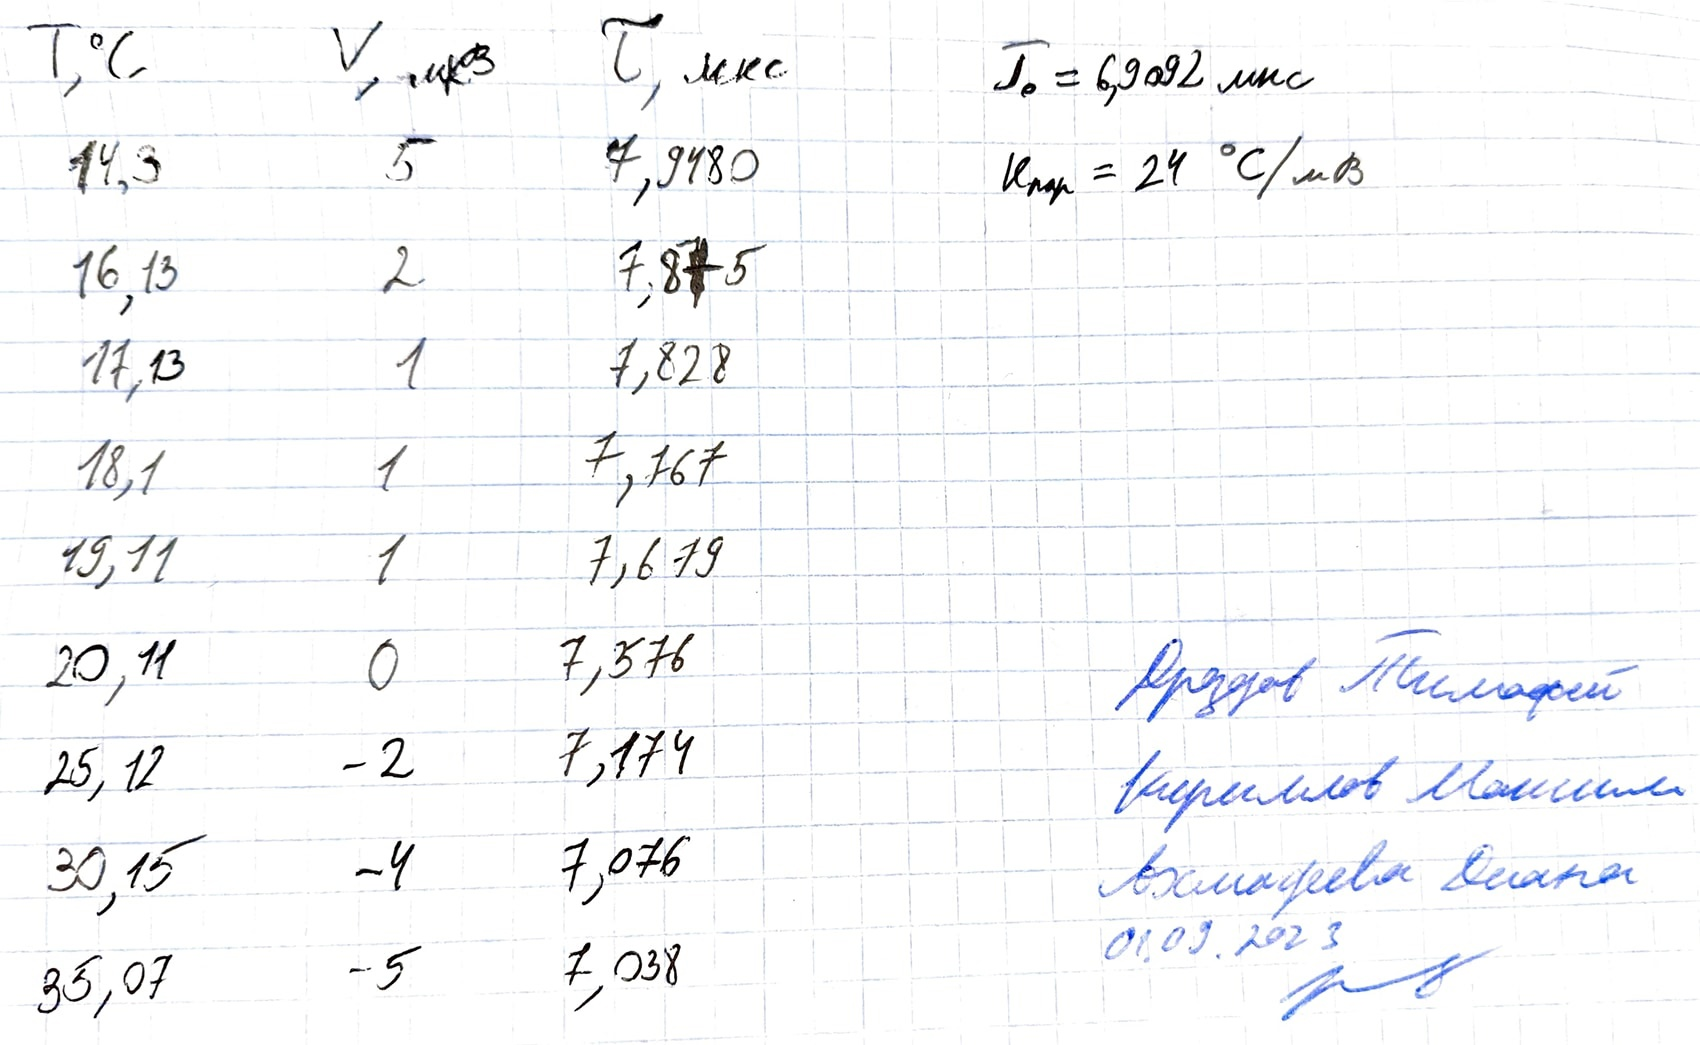
\includegraphics[width=0.8\linewidth]{data.jpg}
\end{figure}

\FloatBarrier

Далее мы рассчитали температуру Т образца с учётом термопары: \[T = T_0 + k * V\]


Затем мы построили график зависимости \[f(T) = \frac{1}{\tau^2 - \tau_0^2}\]

После этого мы экстраполировали полученную пряму к оси абсцисс и определили положение феррамагнитной и парамагнитной точек Кюри.

\FloatBarrier

\begin{figure}[h]
	\centering 
	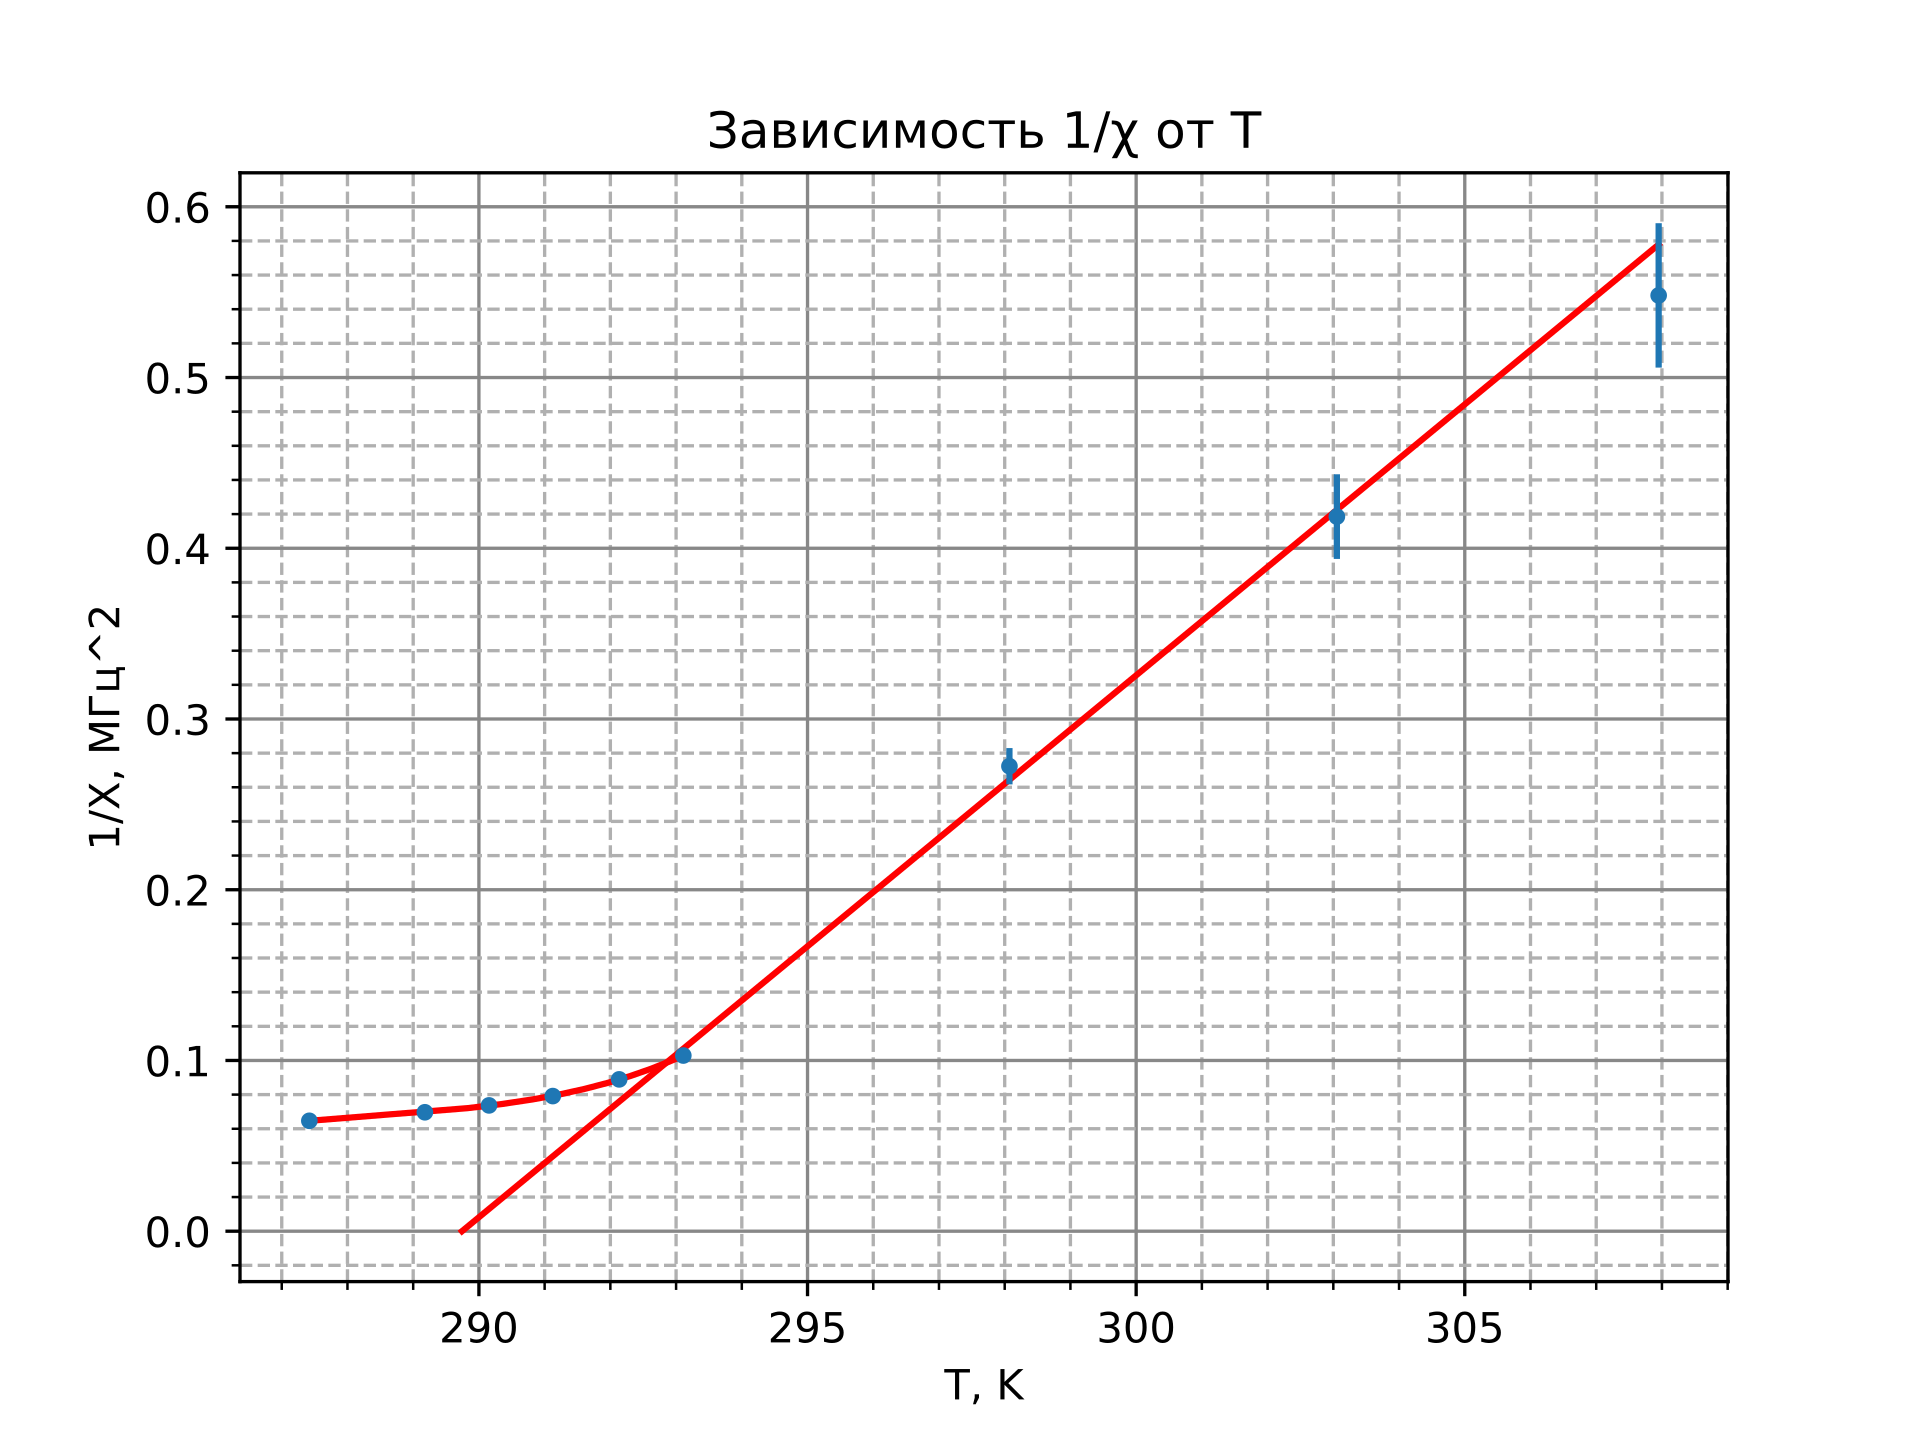
\includegraphics[width=0.8\linewidth]{graph.png}
\end{figure}

\FloatBarrier

Погрешность точек Кюри расчитывалась по формуле \[\sigma \Theta = \sqrt{\sigma T^2 + \sigma V^2}\]
%проверь правильность расчета погрешности

Полученные значения точек Кюри составляют: \[\Theta_p = (289.74 \pm 7.55) ^\circ C\] \[\Theta_k = (279.63 \pm 22.98) ^\circ C\]



\end{document}
